\documentclass{beamer}
\usepackage{movie15}
\begin{document}
\title{Auto Gain: A step to Motion HDR}   
\author{Neal Wadhwa} 
\date{October 22, 2014} 

\frame{\titlepage} 

\frame{\frametitle{Motivation}
\begin{itemize}
\item Make motion magnification is easier to use

\item Eliminate motion gain parameter ($\alpha$) as a first step

\item Introduce an auto-gain
\end{itemize}

}
\frame{\frametitle{Two strategies}
\begin{itemize}
\item After space-time filtering
\item Previous method: multiply by user-specified constant
\begin{tabular}{ccc}
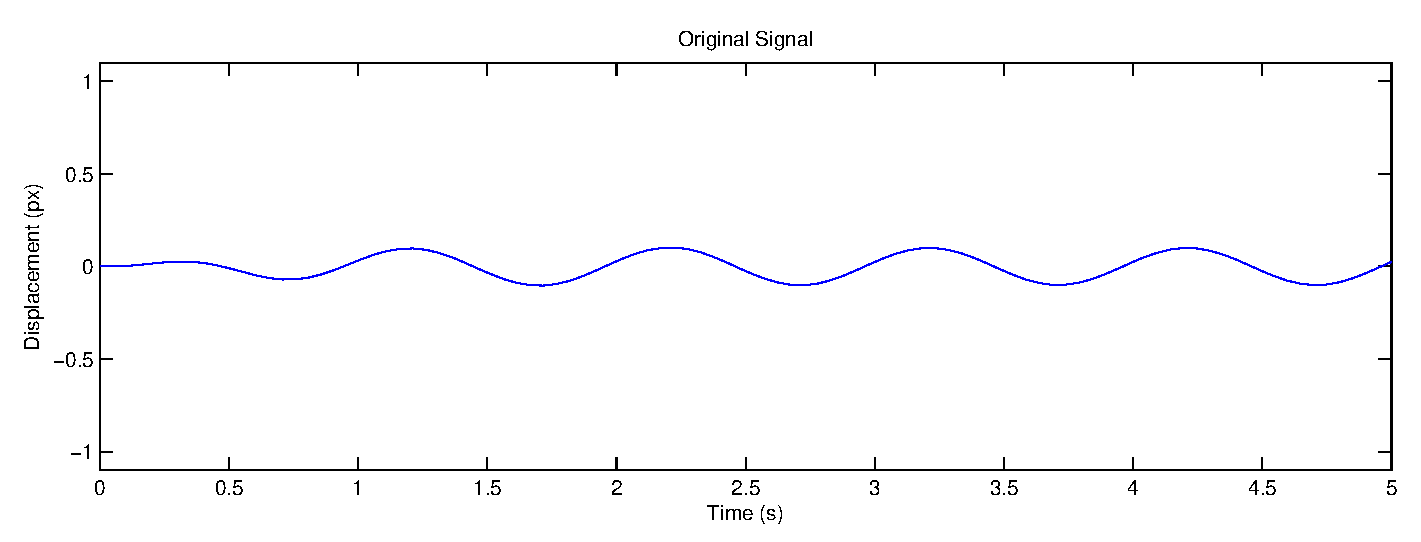
\includegraphics[width=1.5in]{autogain/original.eps} & $\Rightarrow$ & 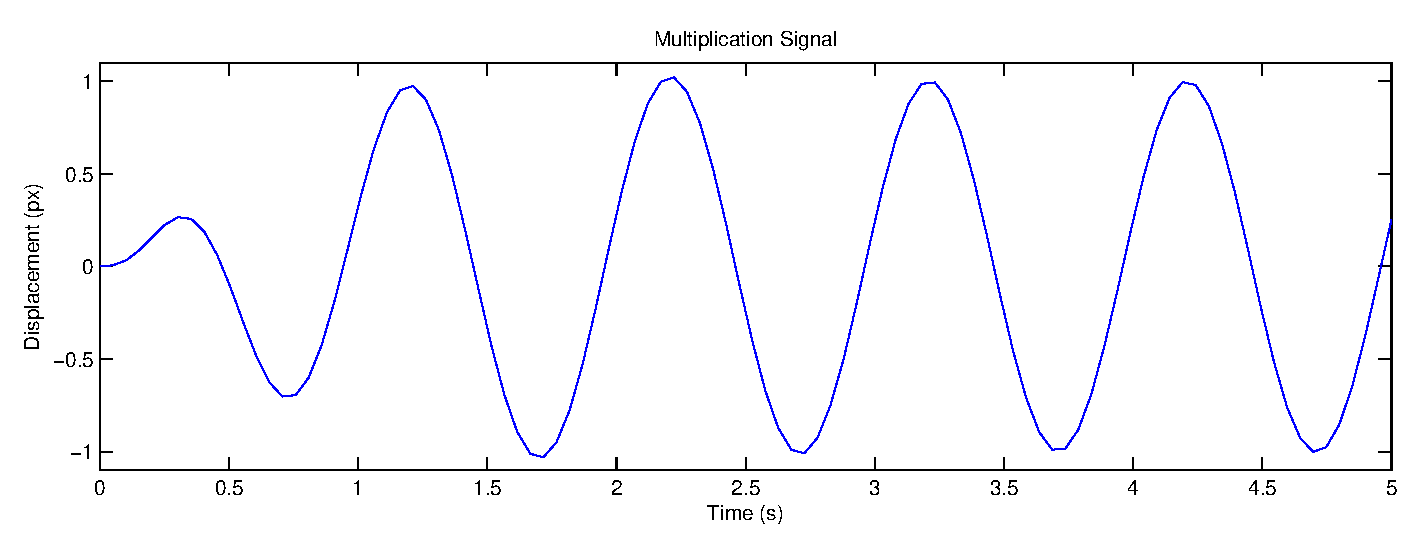
\includegraphics[width=1.5in]{autogain/control.eps}\\
\tiny{Original}  &  & \tiny{Constant multiplier}\\
\end{tabular}

\item Strategy 1: Make phase changes have absolute value 5 px 
\begin{tabular}{ccc}
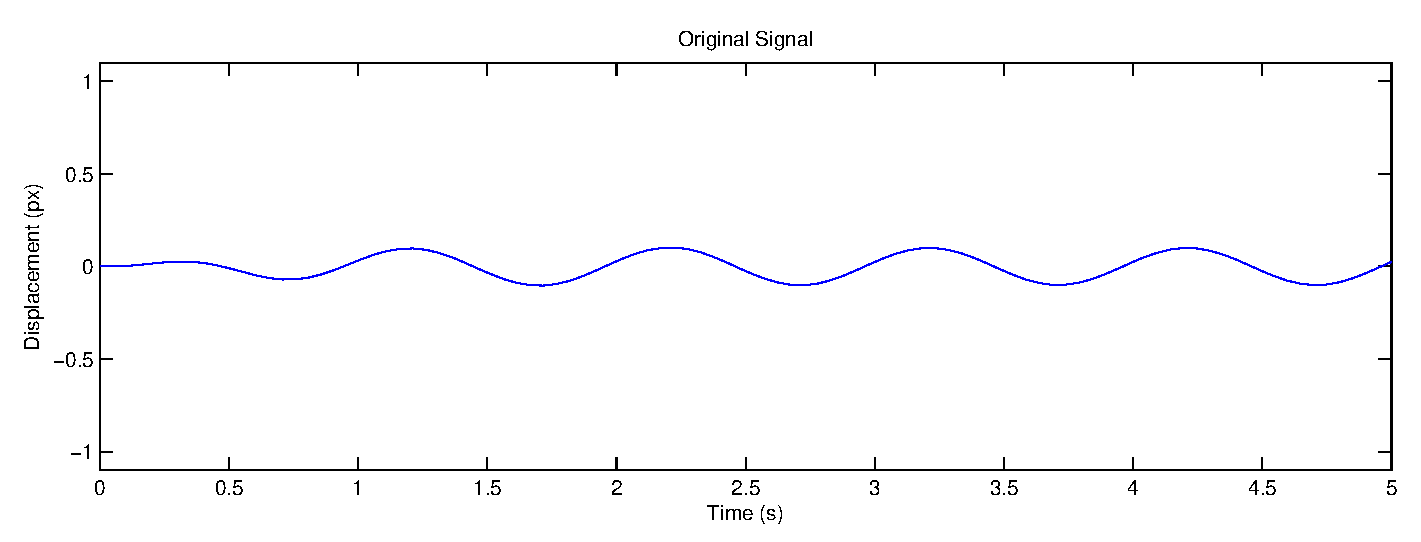
\includegraphics[width=1.5in]{autogain/original.eps} & $\Rightarrow$ & 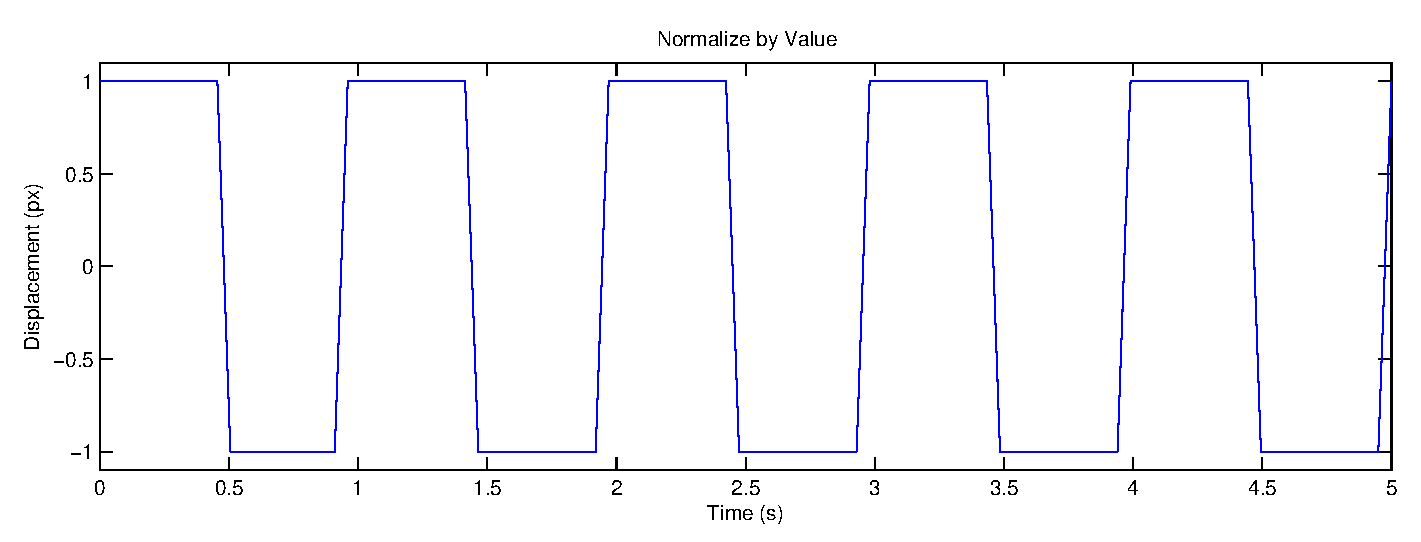
\includegraphics[width=1.5in]{autogain/strategy1.eps}\\
\tiny{Original}  &  & \tiny{Auto-gained}\\
\end{tabular}
\item Strategy 2: Make phase changes have Hilbert transform 5px
\begin{tabular}{ccc}
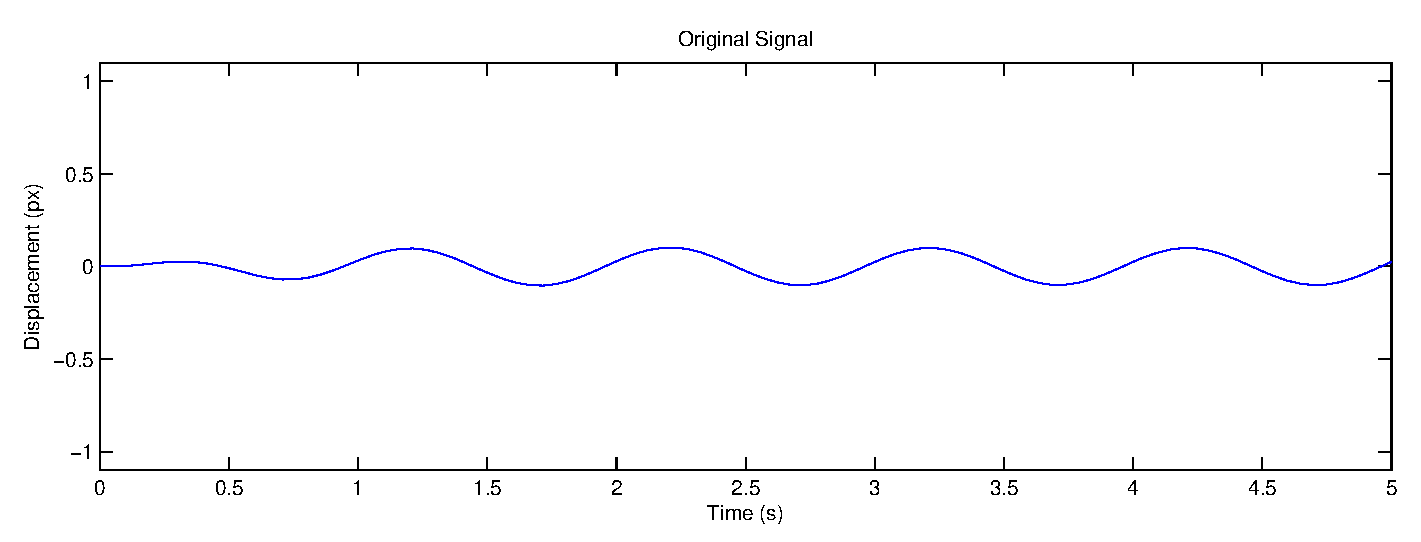
\includegraphics[width=1.5in]{autogain/original.eps} & $\Rightarrow$ & 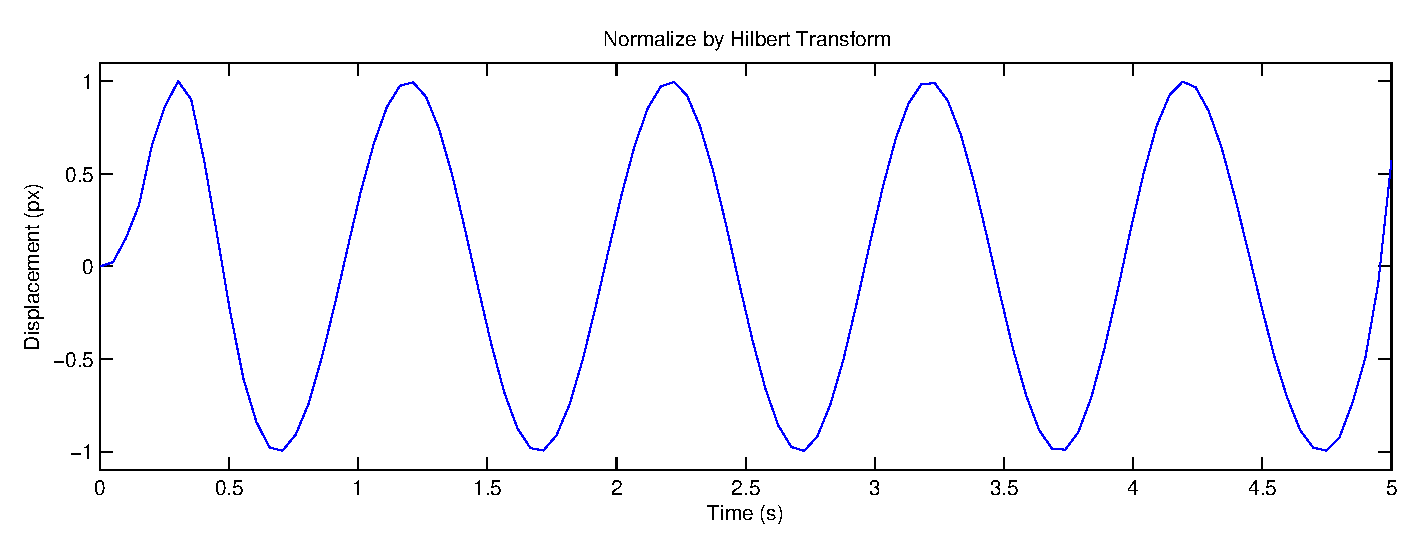
\includegraphics[width=1.5in]{autogain/strategy2.eps}\\
\tiny{Original}  &  & \tiny{Auto-gained}\\
\end{tabular}
\end{itemize}

}

\frame{\frametitle{Details}
\begin{itemize}
\item Uses complex steerable pyramid, not Riesz pyramid

\item Each scale and orientation is processed independently

\item But, each coarser scale has half the max amplitude as the previous one.

\end{itemize}
}

\frame{\frametitle{Column}
\begin{itemize}
\item Uses complex steerable pyramid, not Riesz pyramid

\item Result: \movie{10}{autogain/column.mp4}

\item Pretty good, more or less replicates previous result automatically

\item Strategy 1 is not as good as strategy 2

\end{itemize}
}

\frame{\frametitle{Violin - Best Result}
\begin{itemize}
\item Original, Multiplied by Constant, Auto Gain using Hilbert

\item Result: \movie{10}{autogain/violin.mp4}

\item Better than multiplying by constant

\item Doesn't amplify moving string

\item Bow doesn't move too much

\end{itemize}
}

\frame{\frametitle{Guitar - Worst Result}
\begin{itemize}
\item Original, Multiplied by Constant, Auto Gain using Hilbert

\item Result: \movie{10}{autogain/guitar.mp4}

\item Noise gets amplified like crazy, wiping out all the texture.

\item The string with signal looks good, but everything else is bad

\end{itemize}
}


\frame{\frametitle{1D Noise example}

\begin{tabular}{ccc}
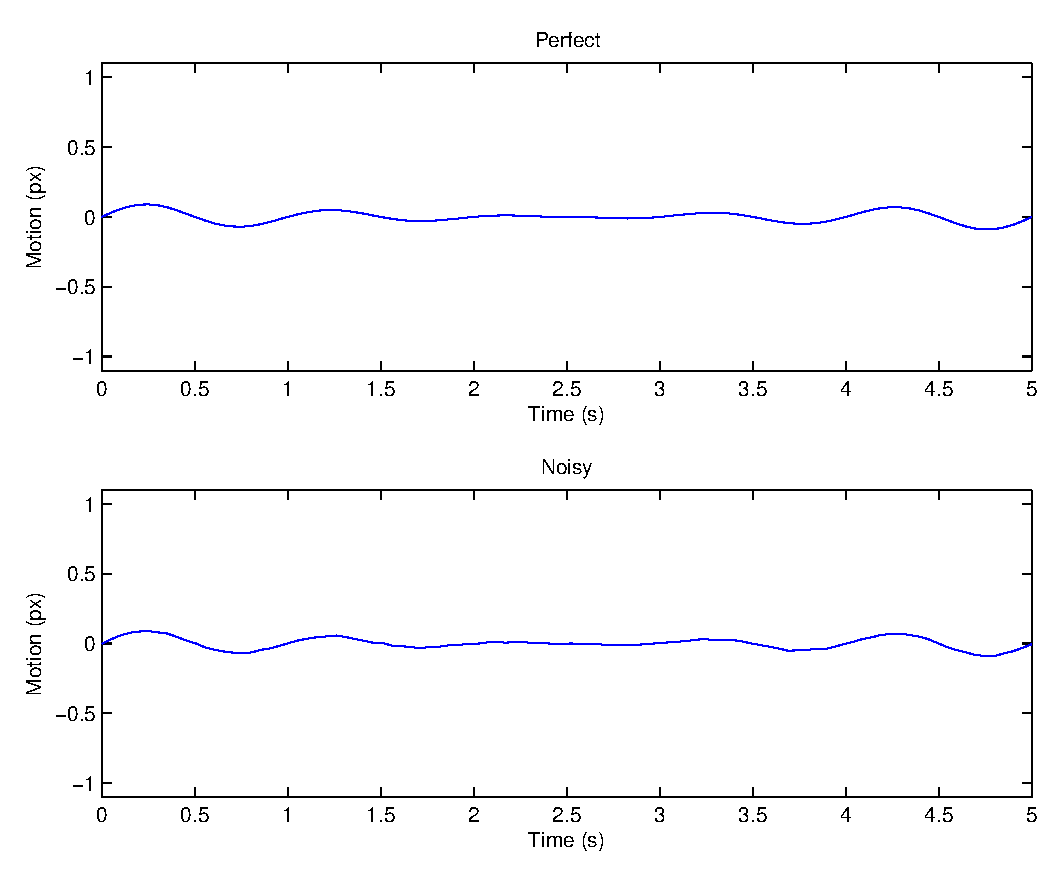
\includegraphics[width=1.3in]{autogain/noiseExamples/original.eps} &
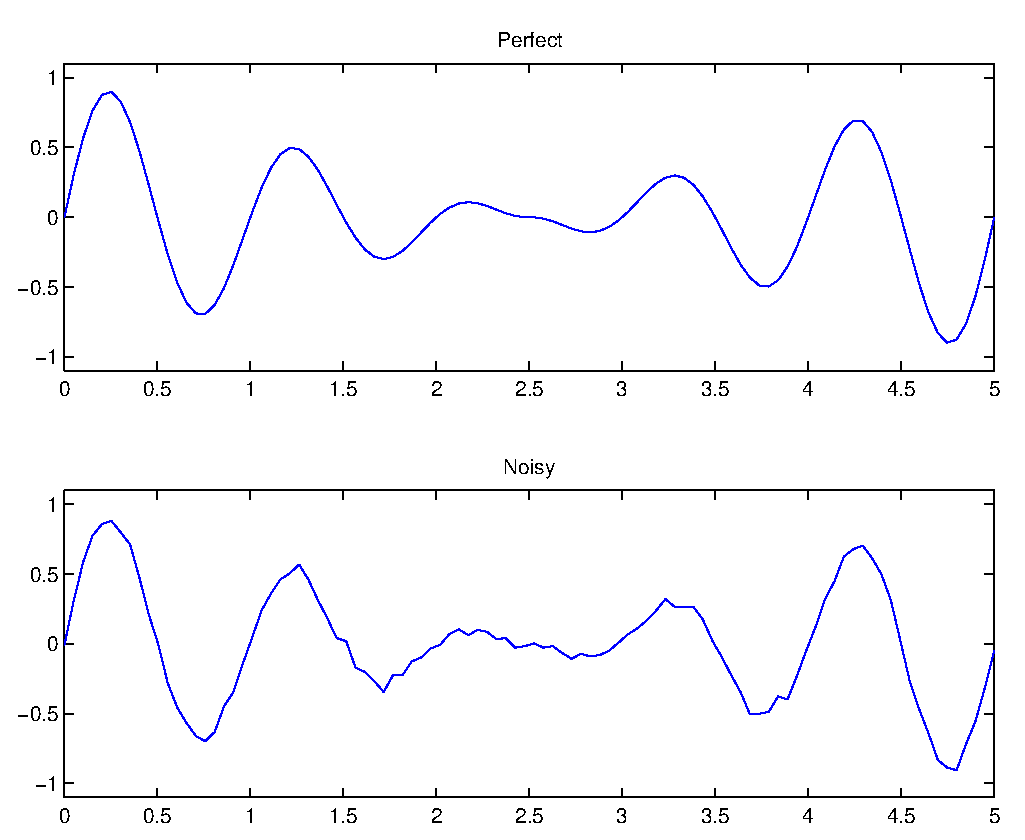
\includegraphics[width=1.3in]{autogain/noiseExamples/control.eps} &
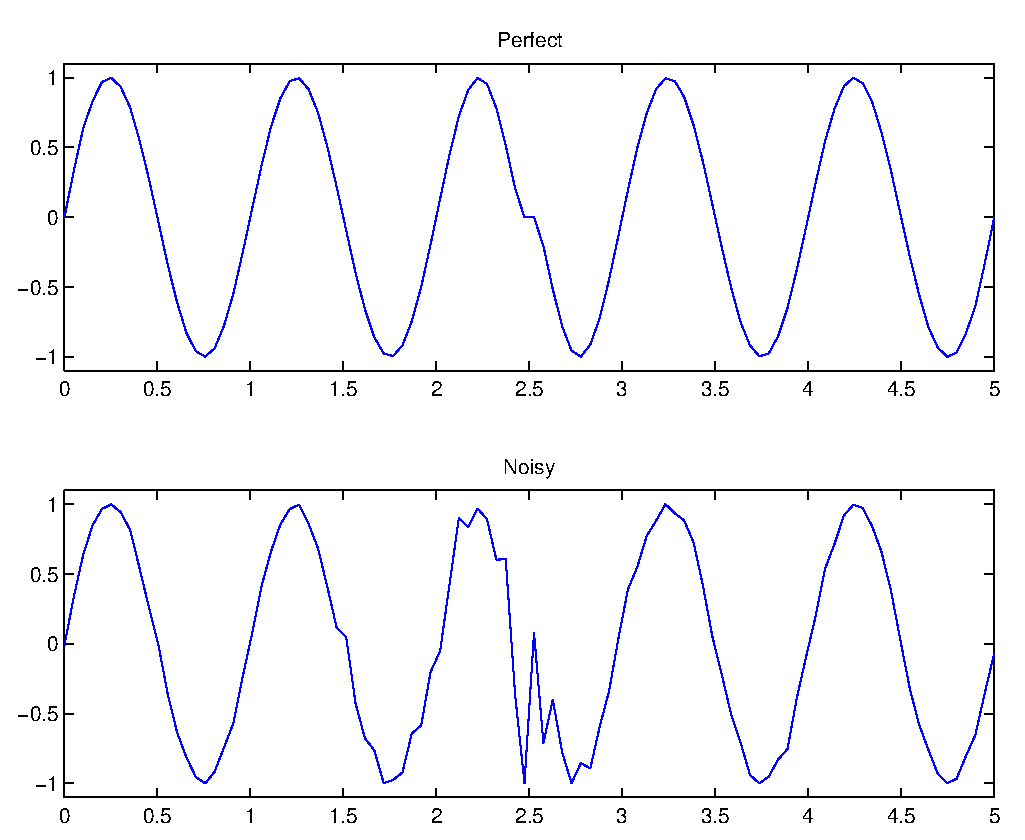
\includegraphics[width=1.3in]{autogain/noiseExamples/hilbert.eps} \\
Original & Multiplied by Constant & Auto gained (Hilbert)\\
\end{tabular}
\begin{itemize}
\item Noise standard deviation of  $0.003$, max signal amplitude $0.1$

\item Noise gets amplified by autogainer, causing problems
\end{itemize}
}



\frame{\frametitle{Future Work}
\begin{itemize}
\item Causal Hilbert transformer (just need amplitude, not pair)
\item What happens to 2d structures, or edges split across orientations?
\item Implement Riesz transform version

\item Reduce auto-gain in presense of noise

\item Can be misleading about relative size of motions, so display gain map?

\end{itemize}
}

\end{document}